\documentclass[11pt]{article}
\usepackage[margin=1in]{geometry}
\usepackage{graphicx}
\usepackage{amsmath}
\begin{document}
\section*{R95 cusp divisors for the two-chart cover}
From the accepted degree-16 ramification fibers and the elliptic base
divisor $\operatorname{div}(u)=[A]+[B]-2[O]$, the transported
overlap functions have complete source divisors
\[
\operatorname{div}(h)=D_O+D_D-2D_B,\qquad
\operatorname{div}(k)=D_O+D_C-2D_A.
\]
Here each $D_X$ has degree 16 and includes the two index-1 and two
index-7 branches above $X$. Both divisors have zero and pole degree 32.

\begin{center}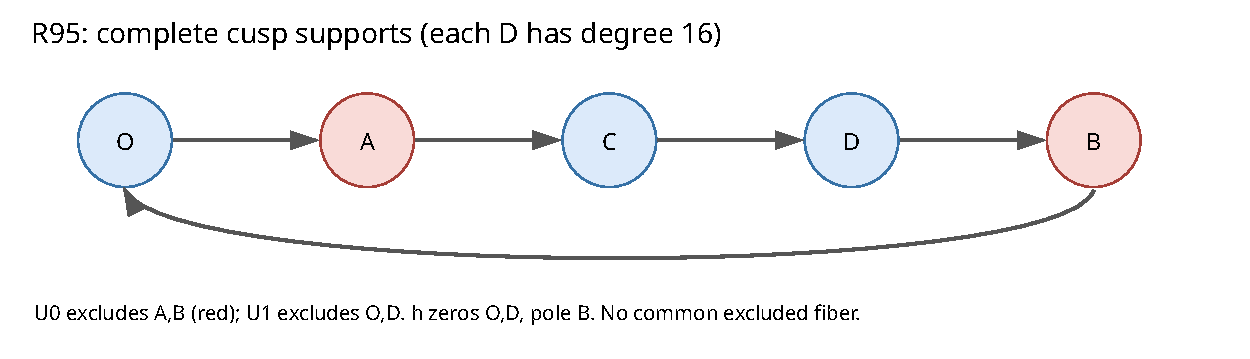
\includegraphics[width=.94\textwidth]{diagram.pdf}\end{center}

On $U_0=X\setminus(D_A\cup D_B)$, $h$ is regular and vanishes exactly
at $D_O\cup D_D$. Hence $U_0\cap U_1=D_{U_0}(h)$ and
$U_0\cup U_1=X$ for $U_1=X\setminus(D_O\cup D_D)$.
The abstract second chart has overlap $D(k)$. R91/R94 check the
transition on its rank-32 algebra. The Lean file checks the finite
cusp permutation and support arithmetic; divisor pullback and the
normal-chart identification use the cited geometric/source inputs.
\end{document}
